
\section{Misconceptions in Some Existing Results}
\label{sec:misconceptions}

This section explains several misconceptions in some existing results by presenting concrete examples to demonstrate their overstatements. These examples are constructed case by case. Therefore, each misconception will be explained by using one specific example. 

\subsection{Incorrect Quantifications of Jitter - Dynamic Self-Suspension}
\label{sec:wrong-jitter-dynamic}

We first explain the existing misconceptions in the literature to quantify the jitter too optimistically for dynamic self-suspending task systems under fixed-priority scheduling. To calculate the worst-case response time of the task $\tau_k$ under analysis, there have been several results in the literature, i.e., \cite{ECRTS-AudsleyB04,RTAS-AudsleyB04,RTCSA-KimCPKH95},  which propose to calculate the worst-case response time $R_k$ of task $\tau_k$ by finding the minimum $R_k$ with
\begin{equation}
R_k = C_k+ S_k+\sum_{\tau_i \in hp(k)}\ceiling{\frac{R_k+S_k}{T_i}} C_i.
\label{eq:dynamic-flawed}
\end{equation}
The term $hp(k)$ is the set of the tasks with higher priority levels than task $\tau_k$. This analysis basically assumes that the jitter of a higher-priority task $\tau_i$ due to self-suspension is at most $S_i$.  Intuitively, it represents the potential internal jitter, \textit{within} an activation of $\tau_i$, i.e., when its execution time $C_i$ is considered by disregarding any time intervals when $\tau_i$ is preempted. 
However, it is not a real jitter in the general cases, because the execution of $\tau_i$ can be pushed further, to be shown in the following example.


Consider the dynamic self-suspending task set presented in Table \ref{tab:counterexample-dynamic-suspension}. 
The analysis in Eq.~(\ref{eq:dynamic-flawed}) would yield $R_3=12$, as illustrated in 
Figure~\ref{fig:counterexample-dynamic}(a). However, the schedule of Figure~\ref{fig:counterexample-dynamic}(b), which is perfectly legal, 
disproves the claim that $R_3=12$, because $\tau_3$ in that case has a response time of $22-5\epsilon$ time units, 
where $\epsilon$ is an arbitrarily small quantity. 

\begin{table}[t]
\begin{center}
\begin{tabular}{|c|r|r|r|}
\hline
$\tau_i$ &      $C_i$   &   $S_i$  &     $T_i$     \\ \hline
$\tau_1$ &       $1$   &     $0$  &       $2$     \\ \hline
$\tau_2$  &      $5$   &     $5$  &      $20$     \\ \hline
$\tau_3$  &      $1$   &     $0$  &  $\infty$     \\ \hline
\end{tabular}
\end{center}
\caption{A set of tasks with dynamic self-suspensions for Section \ref{sec:wrong-jitter-dynamic}.}
\label{tab:counterexample-dynamic-suspension}
\end{table}


\begin{figure}[t]
  \centering
\def\uxfpga{0.4cm} 
\subfloat[]{
    \scalebox{0.8}{
      \begin{tikzpicture}[x=\uxfpga,y=\uy,auto, thick]
        \draw[->] (-6,0) -- coordinate (xaxis) (18,0) node[anchor=north]{$t$};
       \node[anchor=east] at (-6, 0.5) {$\tau_3$};
       \node[anchor=east] at (-6, 2.5) {$\tau_2$};
       \node[anchor=east] at (-6, 4.5) {$\tau_1$};

       \foreach \x in {-6,-4,...,16}{
         \draw[-,below](\x,0) -- (\x,-0.3)
         node[] {\pgfmathtruncatemacro\yi{\x} \yi};
       }

        \draw[->] (0,0) -- (0,1.75);
        \draw[<-,thin,red] (0,1.3) -- (5.3,1.3);
        \draw[->,thin,red] (6.7,1.3) -- (12,1.3);
        \draw[<-,thin,red] (0,1.3) -- (5,1.3);
        \draw[] (12.05,0) -- (12.05,1.5);
        \node[anchor=east,red] at (6.7, 1.39) {$12$};
        \draw[dotted] (12.5,0.5) -- (13.3,0.5); 
        \node[task7, minimum width=\uxfpga, anchor=south west] at (11, 0){\footnotesize};         

        \draw[->] (-5,2) -- (-5,3.75);
        \draw[->] (15,2) -- (15,3.75);
        \draw[dotted] (15.5,2.5) -- (16.3,2.5); 
        \draw[] (-5,2.3) -- (0,2.3);
        \draw[] (-5,2.5) -- (0,2.5);
        \draw[] (-5,2.7) -- (0,2.7);
        \draw[] (0,2) -- (0,3);
        \node[task7, minimum width=\uxfpga, anchor=south west] at (1, 2){\footnotesize};
        \node[task7, minimum width=\uxfpga, anchor=south west] at (3, 2){\footnotesize};
        \node[task7, minimum width=\uxfpga, anchor=south west] at (5, 2){\footnotesize};
        \node[task7, minimum width=\uxfpga, anchor=south west] at (7, 2){\footnotesize};
        \node[task7, minimum width=\uxfpga, anchor=south west] at (9, 2){\footnotesize};
                
        \draw[->] (0,4) -- (0,5.75);
        \draw[->] (2,4) -- (2,5.75);
        \draw[->] (4,4) -- (4,5.75);
        \draw[->] (6,4) -- (6,5.75);
        \draw[->] (8,4) -- (8,5.75);
        \draw[->] (10,4) -- (10,5.75);
        \draw[->] (12,4) -- (12,5.75);
        \draw[->] (14,4) -- (14,5.75);
        \draw[dotted] (15.5,4.5) -- (16.3,4.5);
        \node[task7, minimum width=\uxfpga, anchor=south west] at (0, 4){\footnotesize};
        \node[task7, minimum width=\uxfpga, anchor=south west] at (2, 4){\footnotesize};
        \node[task7, minimum width=\uxfpga, anchor=south west] at (4, 4){\footnotesize};
        \node[task7, minimum width=\uxfpga, anchor=south west] at (6, 4){\footnotesize};
        \node[task7, minimum width=\uxfpga, anchor=south west] at (8, 4){\footnotesize};
        \node[task7, minimum width=\uxfpga, anchor=south west] at (10, 4){\footnotesize};
        \node[task7, minimum width=\uxfpga, anchor=south west] at (12, 4){\footnotesize};
        \node[task7, minimum width=\uxfpga, anchor=south west] at (14, 4){\footnotesize};
 \end{tikzpicture}} }

\subfloat[]{
    \scalebox{0.8}{
      \begin{tikzpicture}[x=\uxfpga,y=\uy,auto, thick]
        \draw[->] (0,0) -- coordinate (xaxis) (36,0) node[anchor=north]{$t$};
       \node[anchor=east] at (0, 0.5) {$\tau_3$};
       \node[anchor=east] at (0, 2.5) {$\tau_2$};
       \node[anchor=east] at (0, 4.5) {$\tau_1$};

       \foreach \x in {0,2,...,34}{
         \draw[-,below](\x,0) -- (\x,-0.3)
         node[] {\pgfmathtruncatemacro\yi{\x} \yi};
       }
       

        \draw[->] (10,0) -- (10,1.75);
        \draw[dotted] (32.5,0.5) -- (33.3,0.5); 
        \draw[<-,thin,red] (10,1.3) -- (19,1.3);
        \draw[->,thin,red] (22.4,1.3) -- (31.4,1.3);
        \node[anchor=east,red] at (22.3, 1.39) {$22-5\varepsilon$};
        \node[task7, minimum width=0.1*\uxfpga, anchor=south east] at (20, 0){\footnotesize}; 
        \draw[] (31,1) -- (31.4,1);
        \draw[] (31,0) -- (31.4,0);
        \draw[] (31,0) -- (31,1);
        \draw[] (31.4,0) -- (31.4,1.5);   
        
             

        \draw[->] (0,2) -- (0,3.75);
        \draw[->] (20,2) -- (20,3.75);
        \draw[dotted] (35.2,2.5) -- (36,2.5); 
        \draw[<-] (1.2,3) --(1.8,3.38);
        \node[anchor=east] at (2.7, 3.5) {$\varepsilon$};
        \draw[<-] (19.85,3) --(19.1,3.39);
        \node[anchor=east] at (19.1, 3.5) {$5\varepsilon$};
        
        \draw[] (1,3) -- (1.2,3);
        \draw[] (1,2) -- (1.2,2);
        \draw[] (1,2) -- (1,3);
        \draw[] (1.2,2) -- (1.2,3);        
        \draw[] (1.2,2.3) -- (2,2.3);
        \draw[] (1.2,2.5) -- (2,2.5);
        \draw[] (1.2,2.7) -- (2,2.7);
        \draw[] (2,2) -- (2,3);
        \draw[] (3,3) -- (3.2,3);
        \draw[] (3,2) -- (3.2,2);
        \draw[] (3,2) -- (3,3);
        \draw[] (3.2,2) -- (3.2,3);        
        \draw[] (3.2,2.3) -- (4,2.3);
        \draw[] (3.2,2.5) -- (4,2.5);
        \draw[] (3.2,2.7) -- (4,2.7);
        \draw[] (4,2) -- (4,3);
        \draw[] (5,3) -- (5.2,3);
        \draw[] (5,2) -- (5.2,2);
        \draw[] (5,2) -- (5,3);
        \draw[] (5.2,2) -- (5.2,3);        
        \draw[] (5.2,2.3) -- (6,2.3);
        \draw[] (5.2,2.5) -- (6,2.5);
        \draw[] (5.2,2.7) -- (6,2.7);
        \draw[] (6,2) -- (6,3);        
        \draw[] (7,3) -- (7.2,3);
        \draw[] (7,2) -- (7.2,2);
        \draw[] (7,2) -- (7,3);
        \draw[] (7.2,2) -- (7.2,3);        
        \draw[] (7.2,2.3) -- (8,2.3);
        \draw[] (7.2,2.5) -- (8,2.5);
        \draw[] (7.2,2.7) -- (8,2.7);
        \draw[] (8,2) -- (8,3);
        \draw[] (9,3) -- (9.2,3);
        \draw[] (9,2) -- (9.2,2);
        \draw[] (9,2) -- (9,3);
        \draw[] (9.2,2) -- (9.2,3);        
        \draw[] (9.2,2.3) -- (10,2.3);
        \draw[] (9.2,2.5) -- (10,2.5);
        \draw[] (9.2,2.7) -- (10,2.7);
        \draw[] (10,2) -- (10,3);
        \node[task7, minimum width=\uxfpga, anchor=south east] at (12, 2){\footnotesize};
        \node[task7, minimum width=\uxfpga, anchor=south east] at (14, 2){\footnotesize};
        \node[task7, minimum width=\uxfpga, anchor=south east] at (16, 2){\footnotesize};
        \node[task7, minimum width=\uxfpga, anchor=south east] at (18, 2){\footnotesize};
        \draw[] (19,3) -- (19.4,3);
        \draw[] (19,2) -- (19.4,2);
        \draw[] (19,2) -- (19,3);
        \draw[] (19.4,2) -- (19.4,3);        
        \draw[] (19.4,2.3) -- (20,2.3);
        \draw[] (19.4,2.5) -- (20,2.5);
        \draw[] (19.4,2.7) -- (20,2.7);
        \node[task7, minimum width=\uxfpga, anchor=south west] at (21, 2){\footnotesize};
        \node[task7, minimum width=\uxfpga, anchor=south west] at (23, 2){\footnotesize};
        \node[task7, minimum width=\uxfpga, anchor=south west] at (25, 2){\footnotesize};
        \node[task7, minimum width=\uxfpga, anchor=south west] at (27, 2){\footnotesize};
        \node[task7, minimum width=\uxfpga, anchor=south west] at (29, 2){\footnotesize};
        \draw[] (30,2.3) -- (35,2.3);
        \draw[] (30,2.5) -- (35,2.5);
        \draw[] (30,2.7) -- (35,2.7);
        \draw[] (35,2) -- (35,3);
        
        \draw[->] (0,4) -- (0,5.75);
        \draw[->] (2,4) -- (2,5.75);
        \draw[->] (4,4) -- (4,5.75);
        \draw[->] (6,4) -- (6,5.75);
        \draw[->] (8,4) -- (8,5.75);
        \draw[->] (10,4) -- (10,5.75);
        \draw[->] (12,4) -- (12,5.75);
        \draw[->] (14,4) -- (14,5.75);
        \draw[->] (16,4) -- (16,5.75);
        \draw[->] (18,4) -- (18,5.75);
        \draw[->] (20,4) -- (20,5.75);
        \draw[->] (22,4) -- (22,5.75);
        \draw[->] (24,4) -- (24,5.75);
        \draw[->] (26,4) -- (26,5.75);
        \draw[->] (28,4) -- (28,5.75);
        \draw[->] (30,4) -- (30,5.75);
        \draw[->] (32,4) -- (32,5.75);
        \draw[->] (34,4) -- (34,5.75);
        \draw[dotted] (34.2,4.5) -- (35,4.5);
        \node[task7, minimum width=\uxfpga, anchor=south west] at (0, 4){\footnotesize};
        \node[task7, minimum width=\uxfpga, anchor=south west] at (2, 4){\footnotesize};
        \node[task7, minimum width=\uxfpga, anchor=south west] at (4, 4){\footnotesize};
        \node[task7, minimum width=\uxfpga, anchor=south west] at (6, 4){\footnotesize};
        \node[task7, minimum width=\uxfpga, anchor=south west] at (8, 4){\footnotesize};
        \node[task7, minimum width=\uxfpga, anchor=south west] at (10, 4){\footnotesize};
        \node[task7, minimum width=\uxfpga, anchor=south west] at (12, 4){\footnotesize};
        \node[task7, minimum width=\uxfpga, anchor=south west] at (14, 4){\footnotesize};
        \node[task7, minimum width=\uxfpga, anchor=south west] at (16, 4){\footnotesize};
        \node[task7, minimum width=\uxfpga, anchor=south west] at (18, 4){\footnotesize};
        \node[task7, minimum width=\uxfpga, anchor=south west] at (20, 4){\footnotesize};
        \node[task7, minimum width=\uxfpga, anchor=south west] at (22, 4){\footnotesize};
        \node[task7, minimum width=\uxfpga, anchor=south west] at (24, 4){\footnotesize};
        \node[task7, minimum width=\uxfpga, anchor=south west] at (26, 4){\footnotesize};
        \node[task7, minimum width=\uxfpga, anchor=south west] at (28, 4){\footnotesize};
        \node[task7, minimum width=\uxfpga, anchor=south west] at (30, 4){\footnotesize};
        \node[task7, minimum width=\uxfpga, anchor=south west] at (32, 4){\footnotesize};

 \end{tikzpicture}}       }
  \caption{Two different schedules for the task set in Table~\ref{tab:counterexample-dynamic-suspension}.}
  \label{fig:counterexample-dynamic}
\end{figure}

%\begin{figure}[t]
%\begin{center}
%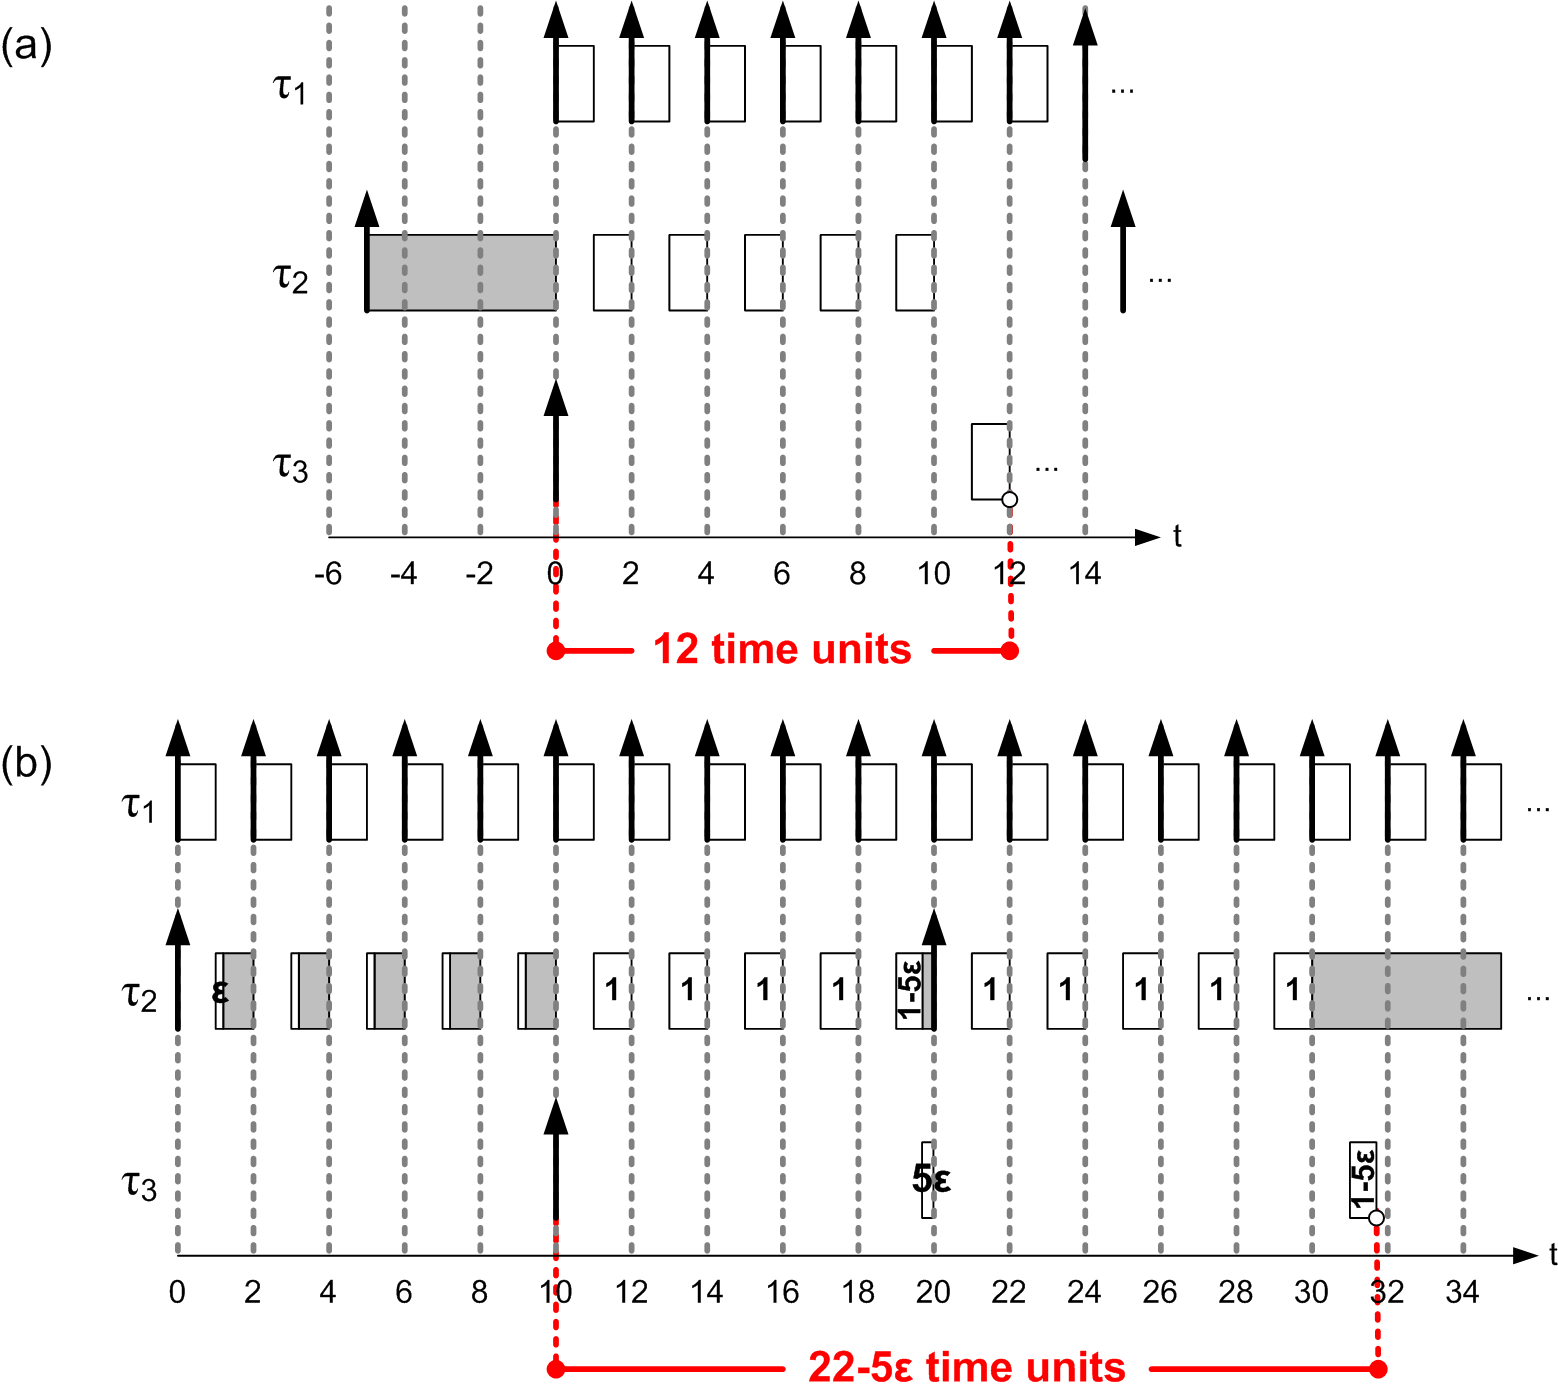
\includegraphics[width=\linewidth]{../figures/CounterexampleDynamicSuspension/counterexample_classic.png}
%\end{center}
%\caption{Two different schedules for the task set in Table~\ref{tab:counterexample-dynamic-suspension}.}
%\label{fig:counterexample-dynamic}
%\end{figure}

{\bf Consequences:} Since the results in \cite{ECRTS-AudsleyB04,RTAS-AudsleyB04,RTCSA-KimCPKH95} are fully based on the analysis in Eq.~(\ref{eq:dynamic-flawed}), the above unsafe example disproves the correctness of their analyses. The authors of the results in \cite{ECRTS-AudsleyB04,RTAS-AudsleyB04} already filed a technical report \cite{BletsasReport2015} to explain in a great detail how to handle this. This misconception was unfortunately applied in \cite{lakshmanan-2009} to analyze the worst-case response time for
partitioned multiprocessor real-time locking protocols, and reused in several other works~\cite{zeng-2011,bbb-2013,yang-2013,kim-2014,han-2014,carminati-2014,yang-2014}. Therefore, this misconception also causes analytical flaws in the above papers. We will explain such consequences in Section~\ref{sec:syn}.
Moreover this counterexample also invalidates the comparison in \cite{RidouardR06}, which compares the schedulability tests from \cite{RTCSA-KimCPKH95} and \cite[Page 164-165]{Liu:2000:RS:518501}, since the result derived from \cite{RTCSA-KimCPKH95} is unsafe.

{\bf Solutions:} It is explained and proved in \cite{huangpass:dac2015,BletsasReport2015} that the worst-case response time of task $\tau_k$ is the minimum $R_k$ with
\begin{equation}
R_k = C_k+ S_k+\sum_{\tau_i \in hp(k)}\ceiling{\frac{R_k+D_i-C_i}{T_i}} C_i,
\label{eq:dynamic-correct}
\end{equation}
for \emph{constrained-deadline} task systems under the assumption that every higher priority task $\tau_i$ in $hp(k)$ can meet their relative deadline constraint. It is also safe to use $\ceiling{\frac{R_k+R_i-C_i}{T_i}}$ instead of $\ceiling{\frac{R_k+D_i-C_i}{T_i}}$ in the above equation if $R_i \leq T_i$.

\subsection{Incorrect Quantifications of Jitter - Segmented Self-Suspension}
\label{sec:wrong-jitter-segmented}


We now explain the existing misconception in the literature to quantify the jitter too optimistically for segmented self-suspending task systems by using fixed-priority scheduling.  The analysis in \cite{RTCSA-BletsasA05} adopts two steps: (1) the computation segments and the self-suspension intervals are reordered such that the computation segments are with decreasing execution time and the suspension intervals are with increasing self-suspending time; and (2) each computation segment has a constant jitter defined by the \emph{early completion of the computation segments and the self-suspension intervals} prior to this computation segment, regardless of the other tasks. 

Instead of going into the detailed mathematical formulations, we will demonstrate the above misconception with the following example listed in Table~\ref{tab:counterexample-segmented}.
In this example, there is only one self-suspending task $\tau_3$. Suppose that all the values of computation time and self-suspension time are all for the actual-case costs. Therefore, both steps mentioned above do not take any effect. The analysis in \cite{RTCSA-BletsasA05} is basically akin to replacing $\tau_3$ with a sporadic task without any jitter or self-suspension, with $C_3=2$ and $D_3=T_3=15$. Therefore, the analysis in \cite{RTCSA-BletsasA05}  concludes that the worst-case response time of task $\tau_4$ is at most $15$ since $C_4+\sum_{i=1}^{3}\ceiling{\frac{15}{T_i}} C_i = 3+ 6 + 4 + 2= 15$.


However, the schedule of Figure \ref{fig:counterexample-segmented} which is perfectly legal, disproves this.
In that schedule, $\tau_1$, $\tau_2$, and $\tau_3$ arrive at $t=0$ and a job of $\tau_4$ arrives at $t=40$ and has a response time of 
$18$ time units.

\begin{table}[t]
\begin{center}
\begin{tabular}{|c||c|r|r|r|}
\hline
$\tau_i$ & $(C_i^1, S_i^1, C_i^2)$   &   $D_i$  &     $T_i$     \\ \hline
$\tau_1$ &  $(2, 0, 0)$                    &     $5$  &       $5$     \\ \hline
$\tau_2$ &  $(2, 0, 0)$                    &    $10$  &      $10$     \\ \hline
$\tau_3$ &  $(1, 5, 1)$            &    $15$  &      $15$     \\ \hline
$\tau_4$ &  $(3, 0, 0)$                   &    $?$  &   $\infty$    \\ \hline     
\end{tabular}
\end{center}
\caption{A set of segmented self-suspending and sporadic real-time tasks for Section~\ref{sec:wrong-jitter-segmented}.}
\label{tab:counterexample-segmented}
\end{table}

\begin{figure}[t]
  \centering
  \def\uxfpga{0.25cm}
    \scalebox{0.77}{
      \begin{tikzpicture}[x=\uxfpga,y=\uy,auto, thick]
        \draw[->] (0,0) -- coordinate (xaxis) (62,0) node[anchor=north]{$t$};
       \node[anchor=east] at (0, 0.5) {$\tau_4$};
       \node[anchor=east] at (0, 2.5) {$\tau_3$};
       \node[anchor=east] at (0, 4.5) {$\tau_2$};
       \node[anchor=east] at (0, 6.5) {$\tau_1$};

       \foreach \x in {0,2,...,60}{
         \draw[-,below](\x,0) -- (\x,-0.3)
         node[] {\pgfmathtruncatemacro\yi{\x} \yi};
       }

        \draw[->] (40,0) -- (40,1.75);
        \draw[] (58.05,1) -- (58.05,1.5);
        \draw[dotted] (58.5,0.5) -- (60,0.5);
        \draw[<-,thin,red] (40,1.3) -- (48,1.3);
        \draw[->,thin,red] (50,1.3) -- (58,1.3);
        \node[anchor=east,red] at (50, 1.39) {18};
        
        \node[task7, minimum width=2*\uxfpga, anchor=south west] at (48, 0){\footnotesize};         
        \node[task7, minimum width=\uxfpga, anchor=south west] at (57, 0){\footnotesize};
        
        \draw[->] (0,2) -- (0,3.75);
        \draw[->] (15,2) -- (15,3.75);
        \draw[->] (30,2) -- (30,3.75);
        \draw[->] (45,2) -- (45,3.75);
        \draw[->] (60,2) -- (60,3.75);
        \draw[dotted] (60.5,2.5) -- (62,2.5); 
        \node[task7, minimum width=\uxfpga, anchor=south west] at (4, 2){\footnotesize};
        \draw[] (5,2.3) -- (10,2.3);
        \draw[] (5,2.5) -- (10,2.5);
        \draw[] (5,2.7) -- (10,2.7);
        \draw[] (10,2) -- (10,3);
        \node[task7, minimum width=\uxfpga, anchor=south west] at (14, 2){\footnotesize};
        \node[task7, minimum width=\uxfpga, anchor=south west] at (17, 2){\footnotesize};
        \draw[] (18,2.3) -- (23,2.3);
        \draw[] (18,2.5) -- (23,2.5);
        \draw[] (18,2.7) -- (23,2.7);
        \draw[] (23,2) -- (23,3);
        \node[task7, minimum width=\uxfpga, anchor=south west] at (24, 2){\footnotesize};
        \node[task7, minimum width=\uxfpga, anchor=south west] at (34, 2){\footnotesize};
        \draw[] (35,2.3) -- (40,2.3);
        \draw[] (35,2.5) -- (40,2.5);
        \draw[] (35,2.7) -- (40,2.7);
        \draw[] (40,2) -- (40,3);
        \node[task7, minimum width=\uxfpga, anchor=south west] at (44, 2){\footnotesize};
        \node[task7, minimum width=\uxfpga, anchor=south west] at (47, 2){\footnotesize};
        \draw[] (48,2.3) -- (53,2.3);
        \draw[] (48,2.5) -- (53,2.5);
        \draw[] (48,2.7) -- (53,2.7);
        \draw[] (53,2) -- (53,3);
        \node[task7, minimum width=\uxfpga, anchor=south west] at (54, 2){\footnotesize};
                
        \draw[->] (0,4) -- (0,5.75);
        \draw[->] (10,4) -- (10,5.75);
        \draw[->] (20,4) -- (20,5.75);
        \draw[->] (30,4) -- (30,5.75);
        \draw[->] (40,4) -- (40,5.75);
        \draw[->] (50,4) -- (50,5.75);
        \draw[->] (60,4) -- (60,5.75);
        \draw[dotted] (60.5,4.5) -- (62,4.5);
        \node[task7, minimum width=2*\uxfpga, anchor=south west] at (2, 4){\footnotesize};
        \node[task7, minimum width=2*\uxfpga, anchor=south west] at (12, 4){\footnotesize};
        \node[task7, minimum width=2*\uxfpga, anchor=south west] at (22, 4){\footnotesize};
        \node[task7, minimum width=2*\uxfpga, anchor=south west] at (32, 4){\footnotesize};
        \node[task7, minimum width=2*\uxfpga, anchor=south west] at (42, 4){\footnotesize};
        \node[task7, minimum width=2*\uxfpga, anchor=south west] at (52, 4){\footnotesize};
        
        \draw[->] (0,6) -- (0,7.75);
        \draw[->] (10,6) -- (10,7.75);
        \draw[->] (20,6) -- (20,7.75);
        \draw[->] (30,6) -- (30,7.75);
        \draw[->] (40,6) -- (40,7.75);
        \draw[->] (50,6) -- (50,7.75);
        \draw[->] (60,6) -- (60,7.75);
        \draw[->] (5,6) -- (5,7.75);
        \draw[->] (15,6) -- (15,7.75);
        \draw[->] (25,6) -- (25,7.75);
        \draw[->] (35,6) -- (35,7.75);
        \draw[->] (45,6) -- (45,7.75);
        \draw[->] (55,6) -- (55,7.75);
        \draw[dotted] (60.5,6.5) -- (62,6.5);
        \node[task7, minimum width=2*\uxfpga, anchor=south west] at (0, 6){\footnotesize};
        \node[task7, minimum width=2*\uxfpga, anchor=south west] at (5, 6){\footnotesize};
        \node[task7, minimum width=2*\uxfpga, anchor=south west] at (10, 6){\footnotesize};
        \node[task7, minimum width=2*\uxfpga, anchor=south west] at (15, 6){\footnotesize};
        \node[task7, minimum width=2*\uxfpga, anchor=south west] at (20, 6){\footnotesize};
        \node[task7, minimum width=2*\uxfpga, anchor=south west] at (25, 6){\footnotesize};
        \node[task7, minimum width=2*\uxfpga, anchor=south west] at (30, 6){\footnotesize};
        \node[task7, minimum width=2*\uxfpga, anchor=south west] at (35, 6){\footnotesize};
        \node[task7, minimum width=2*\uxfpga, anchor=south west] at (40, 6){\footnotesize};
        \node[task7, minimum width=2*\uxfpga, anchor=south west] at (45, 6){\footnotesize};
        \node[task7, minimum width=2*\uxfpga, anchor=south west] at (50, 6){\footnotesize};
        \node[task7, minimum width=2*\uxfpga, anchor=south west] at (55, 6){\footnotesize};        

  \end{tikzpicture}}       
  \caption{A schedule for the task set in Table  \ref{tab:counterexample-segmented}. }
  \label{fig:counterexample-segmented}
\end{figure}

%\begin{figure}[t]
%\begin{center}
%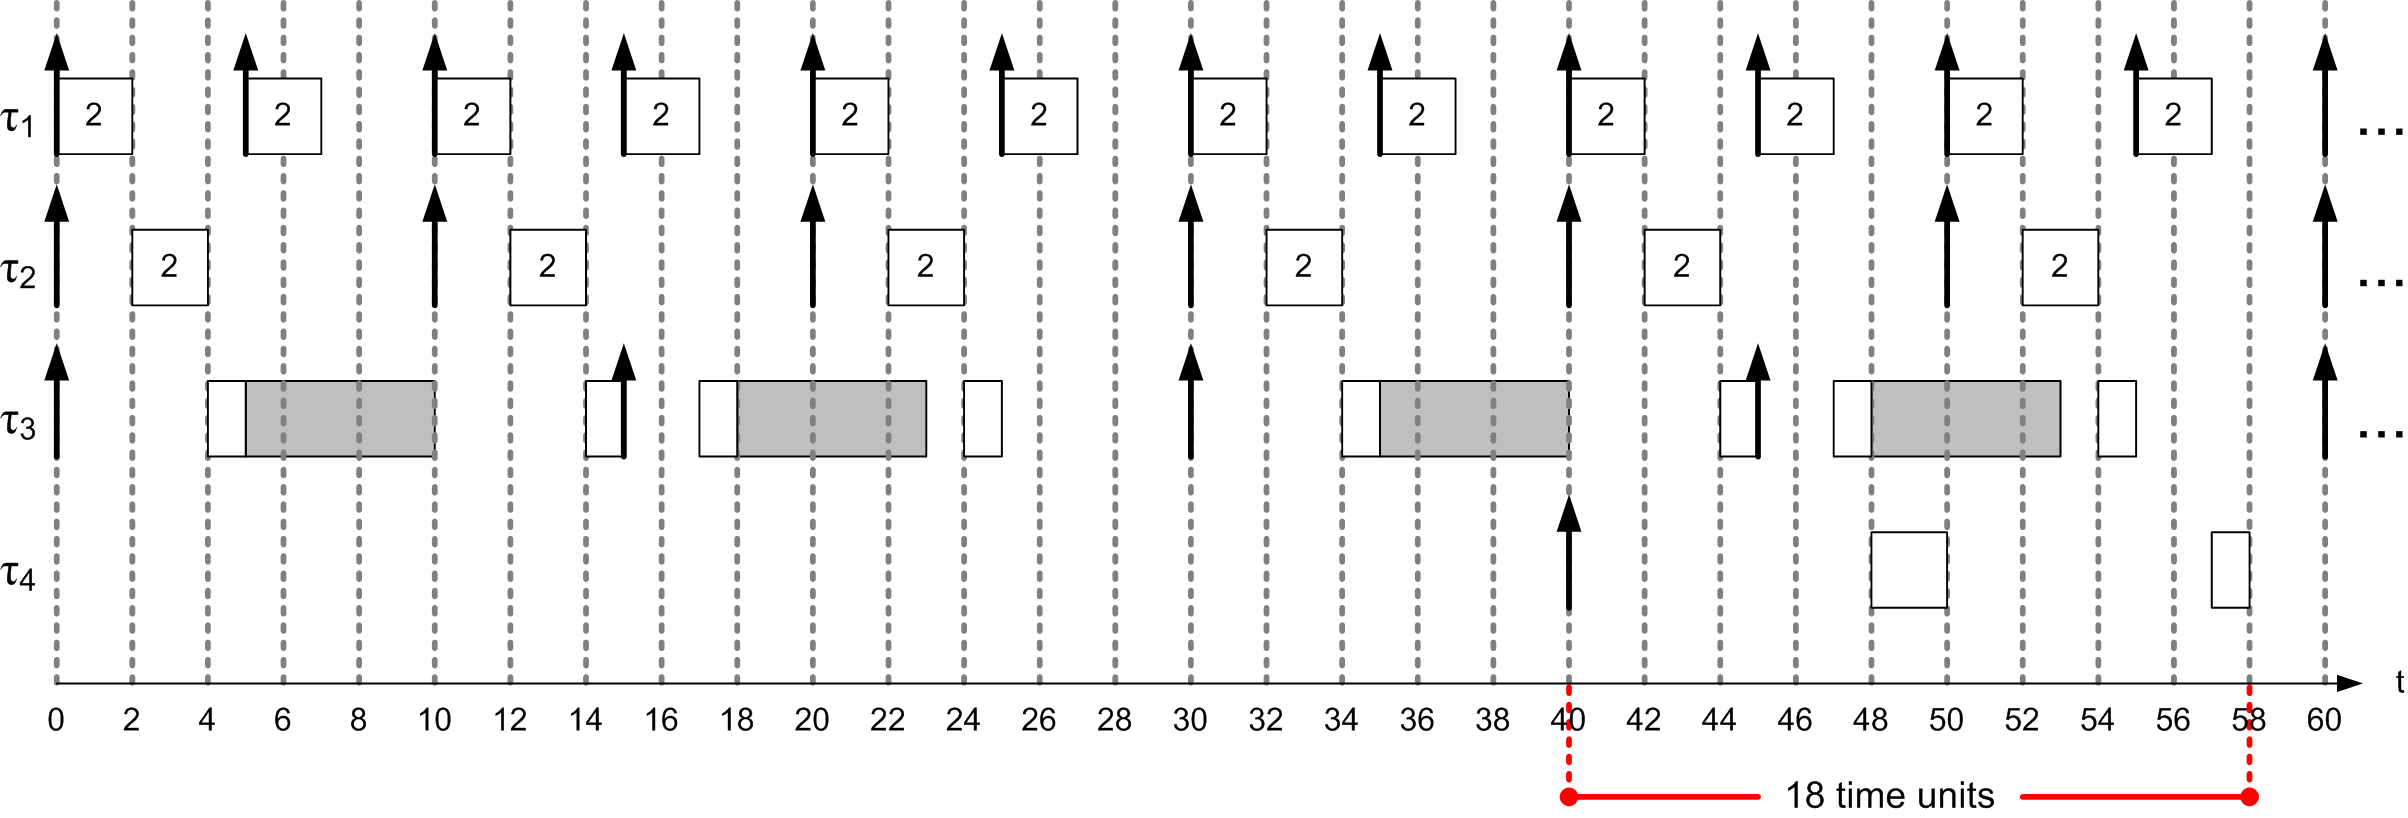
\includegraphics[width=\linewidth]{../figures/CounterexampleSegmentedSuspension/counterexample_synthetic.png}
%\end{center}
%\caption{A schedule for the task set in Table  \ref{tab:counterexample-segmented}. }
%\label{fig:counterexample-segmented}
%\end{figure}

{\bf Consequences:} This example shows that the analysis in \cite{RTCSA-BletsasA05} is flawed.  The authors in \cite{RTCSA-BletsasA05}  already filed a technical report \cite{BletsasReport2015}.

{\bf Solutions:} There is no simple way to fix the error, but quantifying the jitter of a self-suspending task $\tau_i$ with $D_i-C_i$ in Section~\ref{sec:wrong-jitter-dynamic}  remains safe for constrained-deadline task systems since the dynamic self-suspending pattern is more general than a segmented self-suspending pattern.

\subsection{Incorrect Assumptions in Critical Instant with Synchronous Releases}
\label{sec:wrong-critical}

Over the years, it has been well accepted that the characterization of the critical instant for self-suspending tasks is a complex problem. Nevertheless, although the complexity of verifying the existence of a feasible schedule for segmented self-suspending tasks has been proven to be ${\cal NP}$-hard in the strong sense \cite{Ridouard_2004}, the complexity of verifying the schedulability of a task set has only been studied for segmented self-suspending tasks with constrained deadlines scheduled with a fixed-priority scheduling algorithm (see Section~\ref{sec:hardness}), hence leaving hope for the existence of efficient schedulability tests for more constrained systems. 

Following that idea, Lakshmanan and Rajkumar \cite{LR:rtas10} proposed a pseudo-polynomial worst-case response time analysis for one segmented self-suspending (with one self-suspending interval) task $\tau_k$ assuming that 
\begin{itemize}
\item the scheduling algorithm is fixed priority;
\item $\tau_k$ is the lowest priority task;  and
\item all the higher priority tasks are sporadic and non-self-suspending.
\end{itemize}
The analysis, presented in \cite{LR:rtas10}, is based on the notion of critical instant, i.e., an instant at which, considering the state of the system, an execution request for $\tau_k$ will generate the largest response time. This critical instant was defined as follows:
\begin{itemize}
	\item every task releases a job simultaneously with $\tau_k$;
	\item the jobs of higher priority tasks that are eligible to be released during the self-suspension interval of $\tau_k$ are delayed to be aligned with the release of the subsequent computation segment of $\tau_k$; and
	\item all the remaining jobs of the higher priority tasks are released with their minimum inter-arrival time.
\end{itemize}

This definition of the critical instant is very similar to the definition of the critical instant of a non-self-suspending task. Specifically, it is based on the two intuitions that $\tau_k$ suffers the worst-case interference when (i) all higher priority tasks release their first jobs simultaneously with $\tau_k$ and (ii) they all release as many jobs as possible in each computation segment of $\tau_k$. Although intuitive, we provide examples that both statements are wrong, in which the examples already appeared in \cite{ecrts15nelissen}.

\subsubsection{A Counter-Example to the Synchronous Release}

\begin{table} 
\centering
    \begin{tabular}{|c|c|c|}
 \hline
        & $(C_i^1, S_i^1, C_i^2)$ &  $D_i=T_i$\\ 
        \hline
        $\tau_1$ & (1, 0, 0) &  4\\ 
        $\tau_2$ &  (1, 0, 0) & 50  \\ 
        $\tau_3$ & (1, 2, 3) & 100  \\
        \hline
    \end{tabular} 
    \caption{Task parameters for the counter example to the synchronous release of all tasks for Section~\ref{sec:wrong-critical}.}
    \label{table:ex-synch-releases}
\end{table}

\begin{figure}[t]
  \centering
\def\uxfpga{0.4cm} 
    \scalebox{1}{
      \begin{tikzpicture}[x=\uxfpga,y=\uy,auto, thick]
        \draw[->] (0,0) -- coordinate (xaxis) (12,0) node[anchor=north]{$t$};
       \node[anchor=east] at (0, 0.5) {$\tau_3$};
       \node[anchor=east] at (0, 2.5) {$\tau_2$};
       \node[anchor=east] at (0, 4.5) {$\tau_1$};

       \foreach \x in {0,2,...,10}{
         \draw[-,below](\x,0) -- (\x,-0.3)
         node[] {\pgfmathtruncatemacro\yi{\x} \yi};
       }
       
       \node[anchor=east] at (11.5, -1.75) {(a) Release jobs synchronously.};
       \node[anchor=east] at (28, -1.75) {(b) Do not release jobs synchronously.};

        \draw[->] (0,0) -- (0,1.75);
        \draw[dotted] (9.5,0.5) -- (10.3,0.5);
        \draw[<-,thin,red] (0,1.3) -- (3.9,1.3);
        \draw[->,thin,red] (5.1,1.3) -- (9,1.3);
        \draw[] (9.05,0) -- (9.05,1.5);
        \node[anchor=east,red] at (5, 1.39) {$9$}; 
        \node[task7, minimum width=\uxfpga, anchor=south west] at (2, 0){\footnotesize};     
        \node[task7, minimum width=3*\uxfpga, anchor=south west] at (6, 0){\footnotesize};    
        \draw[] (3,0.3) -- (5,0.3);
        \draw[] (3,0.5) -- (5,0.5);
        \draw[] (3,0.7) -- (5,0.7);
        \draw[] (5,0) -- (5,1);
        
        \draw[->] (0,2) -- (0,3.75);
        \draw[dotted] (2.5,2.5) -- (3.3,2.5); 
        \node[task7, minimum width=\uxfpga, anchor=south west] at (1, 2){\footnotesize};
                
        \draw[->] (0,4) -- (0,5.75);
        \draw[dashed,->] (4,4) -- (4,5.75);
        \draw[->] (5,4) -- (5,5.75);
        \draw[->] (9,4) -- (9,5.75);
        \draw[dotted] (10.5,4.5) -- (11.3,4.5);
        \node[task7, minimum width=\uxfpga, anchor=south west] at (0, 4){\footnotesize};
        \node[task7, minimum width=\uxfpga, anchor=south west] at (5, 4){\footnotesize};
        \node[task7, minimum width=\uxfpga, anchor=south west] at (9, 4){\footnotesize};
 

       \draw[->] (15,0) -- coordinate (xaxis) (27,0) node[anchor=north]{$t$};
       \node[anchor=east] at (15, 0.5) {$\tau_3$};
       \node[anchor=east] at (15, 2.5) {$\tau_2$};
       \node[anchor=east] at (15, 4.5) {$\tau_1$};

       \foreach \x in {15,17,...,25}{
         \draw[-,below](\x,0) -- (\x,-0.3)
         node[] {\pgfmathtruncatemacro\yi{\x-15} \yi};
       }

        \draw[->] (15,0) -- (15,1.75);
        \draw[dotted] (25.5,0.5) -- (26.3,0.5); 
        \draw[<-,thin,red] (15,1.3) -- (19.3,1.3);
        \draw[->,thin,red] (20.7,1.3) -- (25,1.3);
        \draw[] (25.05,0) -- (25.05,1.5);
        \node[anchor=east,red] at (20.7, 1.39) {$10$}; 

        \node[task7, minimum width=\uxfpga, anchor=south west] at (16, 0){\footnotesize};     
        \node[task7, minimum width=2*\uxfpga, anchor=south west] at (21, 0){\footnotesize};
        \node[task7, minimum width=\uxfpga, anchor=south west] at (24, 0){\footnotesize};    
        \draw[] (17,0.3) -- (19,0.3);
        \draw[] (17,0.5) -- (19,0.5);
        \draw[] (17,0.7) -- (19,0.7);
        \draw[] (19,0) -- (19,1);
        
        \draw[->] (19,2) -- (19,3.75);
        \draw[dotted] (21.5,2.5) -- (22.3,2.5); 
        \node[task7, minimum width=\uxfpga, anchor=south west] at (20, 2){\footnotesize};
                
        \draw[->] (15,4) -- (15,5.75);
        \draw[->] (19,4) -- (19,5.75);
        \draw[->] (23,4) -- (23,5.75);
        \draw[dotted] (24.5,4.5) -- (25.3,4.5);
        \node[task7, minimum width=\uxfpga, anchor=south west] at (15, 4){\footnotesize};
        \node[task7, minimum width=\uxfpga, anchor=south west] at (19, 4){\footnotesize};
        \node[task7, minimum width=\uxfpga, anchor=south west] at (23, 4){\footnotesize};
 \end{tikzpicture}}     
  \caption{Counter example to the synchronous release of all tasks (by \cite{LR:rtas10}).}
  \label{fig:ex-synch-releases}
\end{figure}

\ifpaper
%\begin{figure}[t]
%  \centering
%\captionsetup[subfigure]{width=\columnwidth}
%  \subfloat[all tasks release a job synchronously.]{\label{fig:ex-phi} }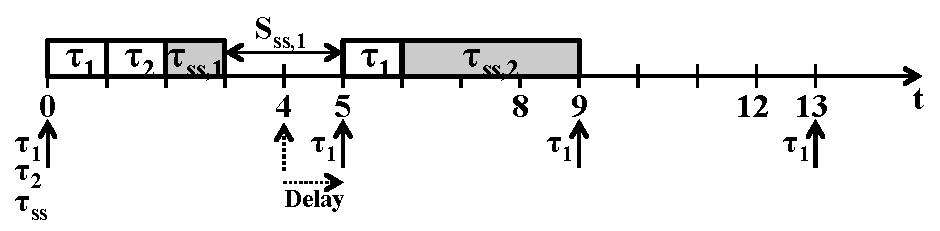
\includegraphics[width=0.85\linewidth]{../figures/ex-phi/ex-phi.pdf} \\
%  \subfloat[all tasks do not release a job synchronously.]{\label{fig:ex-no-phi} }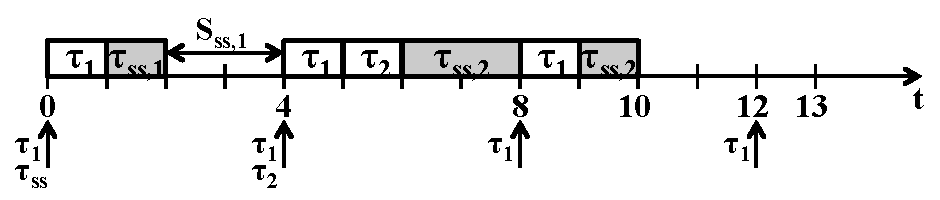
\includegraphics[width=0.85\linewidth]{../figures/ex-no-phi/ex-no-phi}
%  \caption{Counter-example to the synchronous release of all tasks (by \cite{LR:rtas10}).}
%  \label{fig:ex-synch-releases}
%\end{figure}
\fi

Consider three implicit deadline tasks with the parameters presented in Table~\ref{table:ex-synch-releases}. Let us assume that the priorities of the tasks are assigned using the rate monotonic policy (i.e., the smaller the period, the higher the priority). We are interested in computing the worst-case response time of $\tau_3$. Following the definition of the critical instant presented in \cite{LR:rtas10}, all three tasks must release a job synchronously at time $0$. Using the standard response-time analysis for non-self-suspending tasks, we get that the worst-case response time of the first computation region of $\tau_3$ is equal to $R_3^1 = 3$. Because the second job of $\tau_1$ would be released in the self-suspending interval of $\tau_3$ if $\tau_1$ was strictly respecting its minimum inter-arrival time, the release of the second job of $\tau_1$ is delayed so as to coincide with the release of the second computation region of $\tau_3$ (see Figure~\ref{fig:ex-synch-releases}(a)). Considering the fact that the second job of $\tau_2$ cannot be released before time instant $50$ and hence does not interfere with the execution of $\tau_3$, the response time of the second computation segment of $\tau_3$ is thus equal to $R_3^2=4$. In total, the worst-case response time of $\tau_3$ when all tasks release a job synchronously is equal to 
$$R_3 = R_3^1 + S_3^1 + R_3^2 = 3 + 2 +4 = 9$$

Now, let us consider a job release pattern as shown in Figure~\ref{fig:ex-no-phi}. Task $\tau_2$ does not release a job synchronously with task $\tau_3$ but with its second computation segment instead. The response time of the first computation segment of $\tau_3$ is thus reduced to $R_3^1=2$. However, both $\tau_1$ and $\tau_2$ can now release a job synchronously with the second computation segment of $\tau_3$, for which the response time is now equal to $R_3^2=6$ (see Figure~\ref{fig:ex-synch-releases}(b)). Thus, the total response time of $\tau_3$ in a scenario where not all higher priority tasks release a job synchronously with $\tau_3$ is equal to 
$$R_3 = R_3^1 + S_3^1 + R_3^2 = 2+2+6 = 10$$

{\bf Consequences:} To conclude, the synchronous release of all tasks does not necessarily generate the maximum interference for the self-suspending task $\tau_k$ and is thus not always a critical instant for $\tau_k$. 
It was however proven in \cite{ecrts15nelissen} that in the critical instant of a self-suspending task $\tau_k$, every higher priority task releases a job synchronously with the arrival of at least one computation segment of $\tau_k$, but not all higher priority tasks must release a job synchronously with the same computation segment.

{\bf Solutions:} The problem to define the critical instant remains open even for the special case defined above. The approach in \cite{ecrts15nelissen} is an exhaustive search.

\subsection{Counting Highest-Priority Self-Suspending Time to Reduce the Interference}
\label{sec:wrong-highest-priority}

We now present a misconception to handle the highest-priority segmented self-suspension task by using the self-suspension time to reduce its interference to the lower-priority sporadic task systems. 
We consider fixed-priority preemptive scheduling to schedule $n$ self-suspending sporadic real-time tasks on a single processor, in which $\tau_1$ is the highest priority task and $\tau_n$ is the lowest priority task. We focus on constrained-deadline task systems with $D_i \leq T_i$ or implicit-deadline systems with $D_i=T_i$ for $i=1,\ldots,n$.
Let us consider the simplest setting of such a case:
\begin{itemize}
\item there is only one self-suspending task, which is the highest-priority task, i.e., $\tau_1$,
\item the self-suspending time is fixed, i.e., early return of self-suspension has to be controlled, and
\item the actual execution time of the self-suspending task is always equal to its worst-case execution time.
\end{itemize}
Denote this task set as $\Gamma_{1s}$ (as also used in \cite{RTSS-KimANR13}).  Since $\tau_1$ is the highest-priority task, its execution behaviour is static under the above assumptions. The misconception here is to identify the critical instant  (Theorem 2 in \cite{RTSS-KimANR13}) as follows: ``a critical instant occurs when all the tasks are released at the same time if $C_1 +S_1 < C_i  \leq T_1-C_1-S_1 \mbox{ for } i \in\{i|i\in Z^{+} \mbox{ and } 1<i\leq n\}$ is satisfied.'' The misconception here is to use the self-suspension time (if it is long enough) to \emph{reduce} the computation demand of $\tau_i$ for interfering with lower-priority tasks. 


{\it Counterexample of Theorem 2 in \cite{RTSS-KimANR13}:} Let $\epsilon$ be a positive and very small number, i.e., $0 < \epsilon \leq 0.1$. We have three tasks, in which
(1) $C_1= 1+ \epsilon$, $C_1^1 = \epsilon$, $S_1=S_1^1 = 1$, $C_1^2  = 1$, $T_{1} =D_1= 4 + 10 \epsilon$, (2) $C_2 = 2 + 2\epsilon$, $T_2 =D_2= 6$, and (3)
$C_3 = 2 + 2\epsilon$, $T_3 =D_3= 6$. It is clear that $2+\epsilon = C_1+S_1 < C_i = 2+2\epsilon \leq T_1-C_1-S_1 = 2+9\epsilon$ for $i=2,3$. The above theorem states that the worst case is to release all the three tasks together at time $0$ (as shown in Figure~\ref{fig:counterexample-reduce-interf}(a)). The analysis shows that the response time of task $\tau_3$ is at most $5+6\epsilon$. However, if we release task $\tau_1$ at time $0$ and release task $\tau_2$ and task $\tau_3$ at time $1+\epsilon$ (as shown in Figure~\ref{fig:counterexample-reduce-interf}(b)), the response time of the first job of task $\tau_3$ is $6+5\epsilon$. 

\begin{figure}[t]
  \centering
\def\uxfpga{0.4cm} 
    \scalebox{1}{
      \begin{tikzpicture}[x=\uxfpga,y=\uy,auto, thick]
        \draw[->] (0,0) -- coordinate (xaxis) (12,0) node[anchor=north]{$t$};
       \node[anchor=east] at (0, 0.5) {$\tau_3$};
       \node[anchor=east] at (0, 2.5) {$\tau_2$};
       \node[anchor=east] at (0, 4.5) {$\tau_1$};

       \foreach \x in {0,2,...,10}{
         \draw[-,below](\x,0) -- (\x,-0.3)
         node[] {\pgfmathtruncatemacro\yi{\x} \yi};
       }
       
       \node[anchor=east] at (11.5, -1.75) {(a) Release jobs synchronously.};
       \node[anchor=east] at (28, -1.75) {(b) Do not release jobs synchronously.};

        \draw[->] (0,0) -- (0,1.75);
        \draw[->] (6,0) -- (6,1.75);       
        \draw[dotted] (6.5,0.5) -- (7.3,0.5);
        \draw[<-,thin,red] (0,1.3) -- (1.5,1.3);
        \draw[->,thin,red] (4.1,1.3) -- (5.6,1.3);
        \node[anchor=east,red] at (4.2, 1.39) {$5+6\varepsilon$};         
        \draw[] (3.3,1.03) -- (4.8,1.03);
        \draw[] (3.3,0) -- (3.3,1);
        \draw[] (4.8,0) -- (4.8,1);
        \draw[] (5,1.03) -- (5.6,1.03);
        \draw[] (5,0) -- (5,1);
        \draw[] (5.6,0) -- (5.6,1.5);
        
        
        \draw[->] (0,2) -- (0,3.75);
        \draw[->] (6,2) -- (6,3.75);
        \draw[dotted] (6.5,2.5) -- (7.3,2.5); 
        \node[task7, minimum width=\uxfpga, anchor=south west] at (0.2, 2){\footnotesize};
        \draw[] (2.2,2.03) -- (3.3,2.03);
        \draw[] (2.2,3.03) -- (3.3,3.03);
        \draw[] (2.2,2.03) -- (2.2,3.03);
        \draw[] (3.3,2.03) -- (3.3,3.03);
       
                        
        \draw[->] (0,4) -- (0,5.75);
        \draw[->] (4.8,4) -- (4.8,5.75);
        \draw[->] (9.6,4) -- (9.6,5.75);
        \draw[dotted] (10.1,4.5) -- (11,4.5);
        \draw[] (0,5.03) -- (0.2,5.03);
        \draw[] (0,4.03) -- (0.2,4.03);
        \draw[] (0.2,4.03) -- (0.2,5.03);
        \draw[] (0.2,4.3) -- (1.2,4.3);
        \draw[] (0.2,4.5) -- (1.2,4.5);
        \draw[] (0.2,4.7) -- (1.2,4.7);        
        \node[task7, minimum width=\uxfpga, anchor=south west] at (1.2, 4){\footnotesize};
        \draw[] (4.8,5.03) -- (5,5.03);
        \draw[] (4.8,4.03) -- (5,4.03);
        \draw[] (5,4.03) -- (5,5.03);
        \draw[] (5,4.3) -- (6,4.3);
        \draw[] (5,4.5) -- (6,4.5);
        \draw[] (5,4.7) -- (6,4.7);        
        \node[task7, minimum width=\uxfpga, anchor=south west] at (6, 4){\footnotesize};
                
      
       \draw[->] (15,0) -- coordinate (xaxis) (27,0) node[anchor=north]{$t$};
       \node[anchor=east] at (15, 0.5) {$\tau_3$};
       \node[anchor=east] at (15, 2.5) {$\tau_2$};
       \node[anchor=east] at (15, 4.5) {$\tau_1$};



       \foreach \x in {15,17,...,25}{
         \draw[-,below](\x,0) -- (\x,-0.3)
         node[] {\pgfmathtruncatemacro\yi{\x-15} \yi};
       }

        \draw[->] (16.2,0) -- (16.2,1.75);
        \draw[<-,red] (22.2,0) -- (23.6,1.3);
        \node[anchor=east,red] at (25.5, 1.68) {miss};
        \draw[<-,thin,red] (16.2,1.3) -- (18,1.3);
        \draw[->,thin,red] (20.7,1.3) -- (22.6,1.3);
        \node[anchor=east,red] at (20.8, 1.4) {$6+5\varepsilon$};
        \draw[] (19.25,1.03) -- (19.7,1.03);
        \draw[] (19.25,0.03) -- (19.7,0.03);
        \draw[] (19.25,0.03) -- (19.25,1.03);
        \draw[] (19.7,0.03) -- (19.7,1.03);
        \draw[] (19.9,1.03) -- (20.9,1.03);
        \draw[] (19.9,0.03) -- (20.9,0.03);
        \draw[] (19.9,0.03) -- (19.9,1.03);
        \draw[] (20.9,0.03) -- (20.9,1.03);
        \draw[] (22,1.03) -- (22.6,1.03);
        \draw[] (22,0.03) -- (22,1.03);
        \draw[] (22.6,0.03) -- (22.6,1.5);
        
        \draw[->] (16.2,2) -- (16.2,3.75);
        \draw[->] (22.2,2) -- (22.2,3.75);
        \draw[] (17.2,3.03) -- (19.25,3.03);
        \draw[] (17.2,2.03) -- (19.25,2.03);
        \draw[] (17.2,2.03) -- (17.2,3.03);
        \draw[] (19.25,2.03) -- (19.25,3.03);
                
        \draw[->] (15,4) -- (15,5.75);
        \draw[->] (19.8,4) -- (19.8,5.75);
        \draw[->] (24.6,4) -- (24.6,5.75);
        \draw[] (15,5.03) -- (15.2,5.03);
        \draw[] (15,4.03) -- (15.2,4.03);
        \draw[] (15.2,4.03) -- (15.2,5.03);
        \draw[] (15.2,4.3) -- (16.2,4.3);
        \draw[] (15.2,4.5) -- (16.2,4.5);
        \draw[] (15.2,4.7) -- (16.2,4.7);        
        \node[task7, minimum width=\uxfpga, anchor=south west] at (16.2, 4){\footnotesize};
        \draw[] (19.8,5.03) -- (20,5.03);
        \draw[] (19.8,4.03) -- (20,4.03);
        \draw[] (20,4.03) -- (20,5.03);
        \draw[] (20,4.3) -- (21,4.3);
        \draw[] (20,4.5) -- (21,4.5);
        \draw[] (20,4.7) -- (21,4.7);        
        \node[task7, minimum width=\uxfpga, anchor=south west] at (21, 4){\footnotesize};
 \end{tikzpicture}}     
  \caption{Counter example to the synchronous release of Theorem 2 in \cite{RTSS-KimANR13}.}
  \label{fig:counterexample-reduce-interf}
\end{figure}

This misconception also leads to a wrong statement in Theorem 3 in \cite{RTSS-KimANR13}:
\begin{quote}
{\it Theorem 3 in \cite{RTSS-KimANR13}}: For a taskset $\Gamma_{1s}$ with implicit deadlines, $\Gamma_{1s}$ is schedulable if the total utilization of the taskset is less than or equal to $n((2+2\gamma)^{\frac{1}{n}}-1)-k$, where $n$ is the number of tasks in $\Gamma_{1s}$, and $\gamma$ is the ratio of
$S_1$ to $T_1$ and lies in the range of $0$ to $2^{\frac{1}{n-1}}-1$. 
\end{quote}


{\it Counterexample of Theorem 3 in \cite{RTSS-KimANR13}:} Suppose that the self-suspending task $\tau_1$ has two computation segments, with $C_1^1 = C_1-\epsilon$, $C_1^2 = \epsilon$, and $S_1=S_1^1 > 0$ with very small $0 < \epsilon \ll C_1^1$. For such an example, it is pretty trivial that this self-suspending highest-priority task is like a sporadic task, i.e., self-suspension does not matter. 

{\bf Consequences:} These examples show that Theorems 2 and 3 in \cite{RTSS-KimANR13} are flawed.  

{\bf Solutions:} The three assumptions, i.e., one highest-priority segmented self-suspending task, controlled suspension behaviour and controlled execution time  in \cite{RTSS-KimANR13} actually implies that the self-suspending behaviour of task $\tau_1$ can be modeled as several sporadic tasks with the same minimum inter-arrival time. That is, if the $j$-th computation segment of task $\tau_1$ starts its execution at time $t$, the earliest time for this computation segment to be executed again in the next job of task $\tau_1$ is at least $t+T_1$. Therefore, a constrained-deadline task $\tau_k$ can be feasibly scheduled by the fixed-priority scheduling strategy if $C_1+S_1 \leq D_1$ and for $2 \leq k \leq n$
  \begin{equation}
    \label{eq:tda-fixed}
\exists 0 < t \leq D_k, \qquad C_k + \sum_{i=1}^{k-1}\ceiling{\frac{t}{T_i}}C_i \leq t.    
  \end{equation}
This also implies that the utilization bound (for implicit-deadline task systems) is still Liu and Layland bound $n(2^{\frac{1}{n}}-1)$ \cite{Liu_1973}, regardless of the ratio of $S_1/T_1$. 

\subsection{Incorrect Segmented Fixed-Priority Scheduling with Periodic Enforcement}
\label{sec:wrong-periodic}

We now introduce misconceptions to adopt periodic enforcement for segmented self-suspending task systems. As mentioned in Section~\ref{sec:periodic-enforce}, we can set a constant offset to constrain the release time of a computation segment. If this offset is given, each computation segment behaves like a standard sporadic (or periodic) task. Therefore, the schedulability test for sporadic task systems can be directly applied. Since the offsets of two computation segments of a task may be different, one may want to assign each computation segment a \emph{fixed-priority} level.  However, this has to be carefully handled. 

Consider the following example. Task $\tau_1$ has $T_1=D_1=30$ and execution time $C_1=10$ without self-suspension. Task $\tau_2$ has $T_2=D_2=40$, and $C_2^1=5$, $S_2^1=5$, and $C_2^2=16$. Suppose that the offset of the computation segment $C_2^1$ is $0$ and the offset of the computation segment $C_2^2$ is $10$. This setting creates three sporadic tasks.
Suppose that the segmented fixed priority assignment assigns $C_2^1$ the highest priority and $C_2^2$ the lowest priority. It should be clear that the worst-case response time of $C_2^1$ is $5$ and the worst-case response time of $C_1$ is $15$. We focus on the WCRT analysis of $C_2^2$.


Since the two computation segments of task $\tau_2$ should not have any overlap, one may think that during the analysis of the worst-case response time of $C_2^2$, we do not have to consider the computation segment $C_2^1$. The worst-case response time of $C_2^2$ (after its constant offset $10$) for this case is $26$ since $\ceiling{\frac{26}{30}} C_1 + C_2^2 = 26$. 
Since $26+10 < 40$, one may conclude that this enforcement results in a feasible schedule. This analysis is adopted in Section IV in \cite{RTSS-KimANR13} and Section 3 in \cite{DBLP:journals/ieicet/DingTT09}. 

Unfortunately, it is not. Figure~\ref{fig:counterexample-FP-segment-level} provides a concrete schedule, in which the response time of $C_2^2$ is larger than $30$, which implies a deadline miss. In fact, the $5$ units execution time of $C_2^1$ pushes $C_1$ and results in a deadline miss of task $\tau_2$.


\begin{figure}[t]
  \centering
  \def\uxfpga{0.3cm}
    \scalebox{0.91}{
      \begin{tikzpicture}[x=\uxfpga,y=\uy,auto, thick]
        \draw[->] (0,0) -- coordinate (xaxis) (42,0) node[anchor=north]{$t$};
       \node[anchor=east] at (0, 0.5) {$\tau_2$};
       \node[anchor=east] at (0, 2.5) {$\tau_1$};

       \foreach \x in {0,2,...,40}{
         \draw[-,below](\x,0) -- (\x,-0.3)
         node[] {\pgfmathtruncatemacro\yi{\x} \yi};
       }

        \draw[->] (0,0) -- (0,1.75);
        \draw[->] (10,0) -- (10,1.75);
        \draw[] (5,0.3) -- (10,0.3);
        \draw[] (5,0.5) -- (10,0.5);
        \draw[] (5,0.7) -- (10,0.7);
        \draw[] (0,1.3) -- (3.3,1.3);
        \draw[] (6.6,1.3) -- (10,1.3);
        \node[anchor=east] at (6.6, 1.49) {offset};
        \draw[<-,red] (40,0) -- (40,1.2);
        \node[anchor=east,red] at (41.3, 1.49) {miss};
        \node[task7, minimum width=5*\uxfpga, anchor=south west] at (0, 0){\footnotesize $C_2^1$};         
        \node[task7, minimum width=15*\uxfpga, anchor=south west] at (15, 0){\footnotesize $C_2^2$};

        \draw[->] (0,2) -- (0,3.75);
        \draw[->] (30,2) -- (30,3.75);
        \node[task7, minimum width=10*\uxfpga, anchor=south west] at (5, 2){\footnotesize};         
        \node[task7, minimum width=10*\uxfpga, anchor=south west] at (30, 2){\footnotesize};

  \end{tikzpicture}}       
  \caption{A schedule to release the two tasks in Section~\ref{sec:wrong-periodic} simultaneously.}
  \label{fig:counterexample-FP-segment-level}
\end{figure}

%\begin{figure}[t]
%\begin{center}
%   \begin{tikzpicture}[y=\uy, font=\sffamily,thick]
     
       
       
        \begin{scope}[shift={(0,0)}]
       \draw[->] (0,0)node[anchor=east,align=center] {$\tau_2$} -- coordinate (xaxis) (8.5,0);
      	\foreach \x in {3}{
      
	 	\node[task7, minimum width=6*\uy,
			anchor=south west] at ( \x, 0){\footnotesize $C_2^2$};
	}
	\foreach \x in {0}{

      		 \node[task7, minimum width=2*\uy,
anchor=south west] at ( \x, 0){\footnotesize $C_2^1$};
	 	
	}
	
	\foreach \x in {0}{
		\draw[->](\x,0) -- (\x,2)
	 		node[above] {};
	}
	\foreach \x in {2}{
		\draw[->](\x,0) -- (\x,2)
	 		node[above] {};
	}
	
	\foreach \x in {8}{
		\draw[->,red](\x,1.5) node[anchor=south] {\textit{miss}}  -- (\x,0)
			node[] {$\times$};
	 		
	}
	\foreach \x in {0,1,...,8}{
		\draw[-,below](\x,0) -- (\x,-0.1)
node[] {\pgfmathtruncatemacro\yi{5*\x} \yi};

			
	 		
	}
       \end{scope}
    
      \begin{scope}[shift={(0,2.4)}]
   
      	\draw[->](0,0) -- (0,1.5);
%\draw[->](2,0) -- (2,1);
\draw[->](6,0) -- (6,1.5);

	\foreach \x in {1,6}{
       		\node[task7, minimum width=4*\uy,
			anchor=south west] at ( \x, 0){$C_1$};
	 	
	}
	\draw[->] (0,0)node[anchor=east] {$\tau_1$} -- coordinate (xaxis) (8.5,0);


	
	
       \end{scope}
 %\draw[dotted] (10,0) -- (10,3.5);
    %  \draw[dotted] (15,0) -- (15,3.5);
     % \draw [<->] (10,3.5) -- (15,3.5)
     % 	node[anchor=south,pos=0.5] {$carry$-$in$};


      \end{tikzpicture}
%\end{center}
%\caption{A schedule to release the two tasks in Section~\ref{sec:wrong-periodic} simultaneously at time $0$.}
%\label{fig:counterexample-FP-segment-level}
%\end{figure}

{\bf Consequences:} The priority assignment algorithms in \cite{RTSS-KimANR13,DBLP:journals/ieicet/DingTT09} use the above unsafe schedulability test to verify the priority assignments. Therefore, their results are flawed due to the unsafe schedulability test.

{\bf Solutions:} This requires us to revisit the schedulability test of a given segmented fixed-priority priority assignment. This can be observed as a reduction to 
the generalized multiframe (GMF) task model introduced by Baruah et al.~\cite{baruah1999generalized}. A GMF task $G_i$ consisting of $m_i$ frames is characterized by the $3$-tuple $(\vec{C_i},\vec{D_i},\vec{T_i})$, where $\vec{C_i}$,$\vec{D_i}$, and $\vec{T_i}$ are $m_i$-ary vectors $(C_{i}^0,C_{i}^1,...,C_{i}^{m_i-1})$ of execution requirements, $(D_{i}^0,D_{i}^1,...,D_{i}^{m_i-1})$ of relative deadlines, $(T_{i}^0,T_{i}^1,...,T_{i}^{m_i-1})$ of minimum inter-arrival times, respectively.
In fact, from the analysis perspective, a self-suspending task $\tau_i$ under the offset enforcement is equivalent to a GMF task $G_i$,  by considering the computation segments as the frames with different separation times \cite{WC16-suspend-DATE,DBLP:journals/ieicet/DingTT09}.

However, most of the existing fixed-priority scheduling results for the GMF task model assume a unique priority level \emph{per task}. To the best of our knowledge, the only results that can be applied for a unique level \emph{per computation segment} are the utilization-based analysis in \cite{DBLP:journals/corr/ChenHL15b,huang2015mode}. 

% \subsection{Incorrect Scheduling with Slack Enforcement}
% \label{sec:wrong-slack}



%%% Local Variables:
%%% mode: latex
%%% TeX-master: "JRTS/JRTS.tex"
%%% End:
